%
% frobenius.tex
%
% (c) 2021 Prof Dr Andreas Müller, OST Ostschweizer Fachhochschule
%
\begin{frame}[t]
\setlength{\abovedisplayskip}{5pt}
\setlength{\belowdisplayskip}{5pt}
\frametitle{Frobenius-Automorphismus}
\vspace{-20pt}
\begin{columns}[t,onlytextwidth]
\begin{column}{0.48\textwidth}
$\operatorname{Prim}(\Bbbk) = \mathbb{F}_p$
\uncover<2->{%
\begin{block}{Binomial-Koeffizienten}
\vspace{-10pt}
\begin{align*}
\binom{p}{k}
&=
\frac{
{\color{red}p}\cdot(p-1)\cdot(p-2)\cdot\dots\cdot (p-k+1)
}{
1\cdot2\cdot3\cdot\dots\cdot k
}
\intertext{{\color{red}$p$} wird nicht gekürzt wegen}
\uncover<3->{1&\not\equiv 0 \mod p}\\
\uncover<3->{2&\not\equiv 0 \mod p}\\
\uncover<3->{ &\phantom{a}\vdots}\\
\uncover<3->{k&\not\equiv 0 \mod p}
\end{align*}
\vspace{-10pt}
\end{block}}
\vspace{-5pt}
\uncover<4->{%
\begin{block}{Frobenius-Authomorphismus}
\vspace{-10pt}
\begin{align*}
\uncover<5->{(x+y)^{p\phantom{\mathstrut^n}}
&=
x^{p\phantom{\mathstrut}^n}+y^{p\phantom{mathstrut^n}}}
\\
\uncover<6->{(x+y)^{p^n} &= x^{p^n}+y^{p^n}}
\end{align*}
\end{block}}
\end{column}
\begin{column}{0.48\textwidth}
\begin{block}{Pascal-Dreieck}
\begin{center}
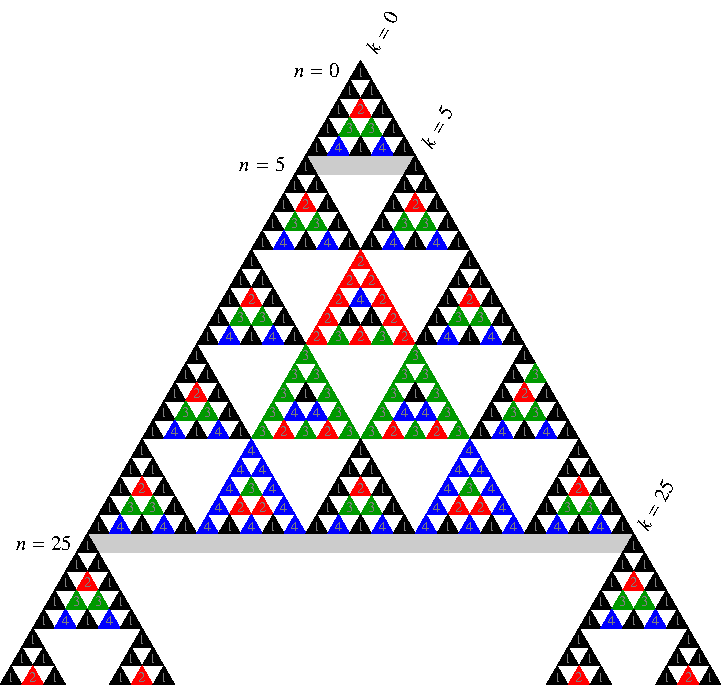
\includegraphics[width=\textwidth]{../../buch/chapters/30-endlichekoerper/images/binomial5.pdf}
\end{center}
\end{block}
\end{column}
\end{columns}
\end{frame}
